\documentclass[aspectratio=169]{beamer}

\usetheme{Madrid}
\usecolortheme{default}

\usepackage[utf8]{inputenc}
\usepackage[T1]{fontenc}
\usepackage[brazil]{babel}
\usepackage{graphicx}
\usepackage{hyperref}
\usepackage{xcolor}
\usepackage{booktabs}
\usepackage{listings}

\definecolor{oceanblue}{RGB}{0,74,119}
\definecolor{oceanlight}{RGB}{219,238,244}
\definecolor{oceangreen}{RGB}{0,120,110}

\setbeamercolor{structure}{fg=oceanblue}
\setbeamercolor{frametitle}{fg=white,bg=oceanblue}
\setbeamercolor{title}{fg=white,bg=oceanblue}
\setbeamercolor{block title}{fg=white,bg=oceangreen}
\setbeamercolor{block body}{bg=oceanlight}

\lstset{
  basicstyle=\ttfamily\small,
  breaklines=true,
  frame=single,
  backgroundcolor=\color{gray!8}
}

\IfFileExists{curso-beamer.sty}{\usepackage{curso-beamer}}{}


\title[Formatos, Metadados e Vocabulários]{Aula 1 --- Formatos de Dados, Metadados e Vocabulários}
\subtitle{Arquiteturas Cloud-Native e Formatos Modernos de Dados para Oceanografia Operacional,\\
Clima e Meteorologia em Escala de Múltiplos Terabytes (Arq-Cloud)}
\author{Tobias Ferreira}
\institute{Instituto Nacional de Pesquisas Oceânicas (INPO)}
\date{01/09/2026}

\begin{document}

% ------------------------------------------------
\begin{frame}[plain,noframenumbering]
  \titlepage
\end{frame}

% ------------------------------------------------
\begin{frame}{Onde esta aula se encaixa?}
\Large
Antes de falar sobre cloud-native, Zarr, Dask e object storage, precisamos responder uma pergunta mais básica:

\vspace{0.5cm}

\begin{block}{Pergunta central}
Como representamos dados ambientais de forma que humanos e máquinas consigam entender, encontrar, reutilizar e processar esses dados corretamente?
\end{block}

\vspace{0.3cm}

\centering
\textbf{Formato sem metadados vira apenas bytes. Metadados sem padrão viram ambiguidade.}
\end{frame}

% ------------------------------------------------
\begin{frame}{Objetivos da aula}
Ao final desta aula, você deverá conseguir:

\begin{itemize}
  \item reconhecer formatos comuns em oceanografia e meteorologia, como NetCDF, GRIB, BUFR e Zarr;
  \item explicar o que são metadados e por que eles são essenciais para descoberta e reúso;
  \item descrever o papel dos vocabulários controlados na padronização de termos;
  \item identificar padrões importantes, como CF, ISO 19115, INSPIRE, MEDIN e NERC NVS;
  \item relacionar formatos tradicionais com formatos cloud-native, como Zarr.
\end{itemize}
\end{frame}

% ------------------------------------------------
\begin{frame}{Perguntas que vamos responder}
\Large
\begin{itemize}
  \item Quais formatos são usados para armazenar dados de oceano e atmosfera?
  \item O que é metadado e como ele ajuda outras pessoas a entenderem meus dados?
  \item Por que vocabulário controlado é melhor do que texto livre?
  \item Quais padrões devo conhecer ao publicar dados ambientais?
  \item Como tudo isso se conecta a formatos modernos como Zarr?
\end{itemize}
\end{frame}

% ------------------------------------------------
\begin{frame}{Por que formatos e metadados importam?}
\Large
Quando trabalhamos com dados ambientais, não armazenamos apenas números.

\vspace{0.4cm}

Também precisamos codificar o \textbf{significado}:

\begin{itemize}
  \item o que foi medido;
  \item onde e quando foi medido;
  \item como foi medido ou processado;
  \item quais unidades, coordenadas e métodos foram usados;
  \item como o dado deve ser interpretado e reutilizado.
\end{itemize}
\end{frame}

% ------------------------------------------------
\begin{frame}{Dois níveis do problema}
\begin{columns}
\column{0.5\textwidth}
\begin{block}{Formato}
Define como dados e metadados são organizados fisicamente.
\end{block}

\begin{itemize}
  \item arrays ou tabelas;
  \item grades ou vetores;
  \item binário ou texto;
  \item arquivo único ou coleção;
  \item legado ou cloud-native.
\end{itemize}

\column{0.5\textwidth}
\begin{block}{Semântica}
Define o significado dos dados.
\end{block}

\begin{itemize}
  \item nomes de variáveis;
  \item unidades;
  \item coordenadas;
  \item sistema de referência;
  \item qualidade e proveniência;
  \item termos controlados.
\end{itemize}
\end{columns}
\end{frame}

% ------------------------------------------------
\begin{frame}{Famílias de formatos ambientais}
\begin{columns}
\column{0.48\textwidth}
\begin{itemize}
  \item formatos de arrays auto-descritivos;
  \item formatos operacionais da WMO;
  \item formatos raster e vetoriais para GIS;
  \item formatos tabulares e colunares;
  \item formatos JSON/XML para catálogos e APIs.
\end{itemize}

\vspace{0.2cm}

\begin{block}{Foco do curso}
Dados multidimensionais de oceano, clima e meteorologia.
\end{block}

\column{0.52\textwidth}
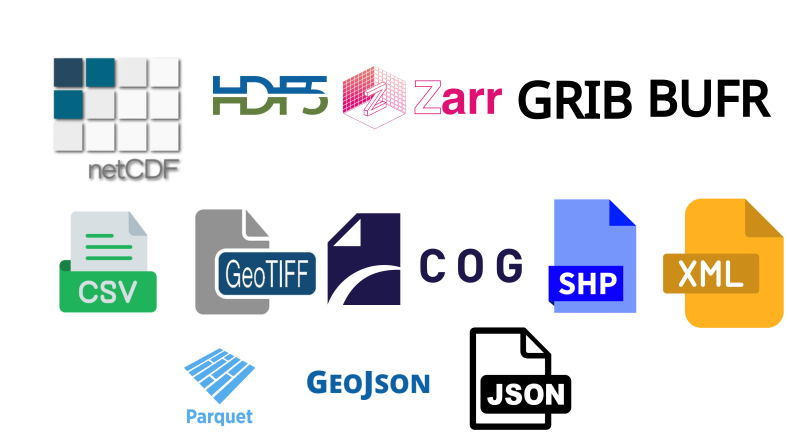
\includegraphics[width=\textwidth]{../episodes/fig/file_formats.png}
\end{columns}
\end{frame}

% ------------------------------------------------
\begin{frame}{Formatos auto-descritivos de arrays}
\begin{table}
\centering
\small
\begin{tabular}{lll}
\toprule
Formato & Uso comum & Ideia principal \\
\midrule
NetCDF & Clima, oceano, reanálise & Arrays + dimensões + atributos \\
HDF5 & Satélite, modelos, ciência & Estrutura hierárquica de grupos \\
Zarr & Dados grandes e cloud-native & Arrays em chunks e acesso paralelo \\
\bottomrule
\end{tabular}
\end{table}

\vspace{0.4cm}

\begin{block}{Por que isso importa?}
Esses formatos carregam dados e metadados estruturais no mesmo dataset: dimensões, variáveis, unidades, coordenadas e atributos.
\end{block}
\end{frame}

% ------------------------------------------------
\begin{frame}{NetCDF}
\begin{itemize}
  \item Formato binário, independente de máquina, muito usado para dados científicos orientados a arrays.
  \item Amplamente adotado em oceanografia, clima e meteorologia.
  \item Armazena variáveis, dimensões, coordenadas e atributos.
  \item Frequentemente usado com convenções CF para tornar os metadados interpretáveis por ferramentas científicas.
\end{itemize}

\vspace{0.4cm}

\begin{block}{Exemplo}
\texttt{sea\_surface\_temperature.nc} contendo latitude, longitude, tempo, temperatura da superfície do mar, unidades e outros metadados.
\end{block}
\end{frame}

% ------------------------------------------------
\begin{frame}{HDF5}
\begin{itemize}
  \item Formato auto-descritivo para datasets grandes e complexos.
  \item Organiza dados em uma estrutura hierárquica, parecida com diretórios.
  \item Usa grupos, datasets e atributos.
  \item Muito comum em produtos de satélite, observações complexas e saídas de modelos.
\end{itemize}

\vspace{0.4cm}

\begin{block}{Exemplo}
\texttt{satellite\_observations.h5} com grupos separados para geolocalização, medições, flags de qualidade e metadados.
\end{block}
\end{frame}

% ------------------------------------------------
\begin{frame}{Zarr}
\begin{itemize}
  \item Formato para arrays N-dimensionais divididos em \textbf{chunks}.
  \item Funciona bem com object storage e acesso remoto.
  \item Permite leitura parcial e processamento paralelo.
  \item Pode representar dados geoespaciais usando convenções como GeoZarr e conceitos do modelo comum de dados da Unidata.
\end{itemize}

\vspace{0.4cm}

\begin{block}{Exemplo}
\texttt{ocean\_model.zarr} com temperatura, salinidade e velocidade indexadas por tempo, profundidade, latitude e longitude.
\end{block}
\end{frame}

% ------------------------------------------------
\begin{frame}{Formatos de troca da WMO}
\begin{columns}
\column{0.5\textwidth}
\begin{block}{GRIB}
Formato binário compacto para campos meteorológicos em grade, muito usado em previsão numérica do tempo.
\end{block}

\begin{itemize}
  \item eficiente para disseminação operacional;
  \item baseado em mensagens;
  \item metadados codificados em tabelas.
\end{itemize}

\column{0.5\textwidth}
\begin{block}{BUFR}
Formato binário flexível e orientado por tabelas para observações meteorológicas e oceanográficas.
\end{block}

\begin{itemize}
  \item usado para satélites, aeronaves e perfis;
  \item representa muitos tipos de observação;
  \item pode carregar informação de qualidade.
\end{itemize}
\end{columns}
\end{frame}

% ------------------------------------------------
\begin{frame}{Outros formatos que aparecem no fluxo}
\begin{table}
\centering
\small
\begin{tabular}{lll}
\toprule
Formato & Tipo & Uso típico \\
\midrule
CSV / ASCII & Tabela simples & Dados pequenos, inspeção manual \\
GeoTIFF / COG & Raster 2D & Mapas, sensoriamento remoto \\
GeoJSON & Vetor JSON & Footprints, regiões, APIs \\
Shapefile & Vetor GIS & Pontos, linhas e polígonos \\
Parquet / GeoParquet & Colunar & Analytics e grandes tabelas \\
XML / JSON & Documento & Metadados, catálogos e APIs \\
\bottomrule
\end{tabular}
\end{table}

\vspace{0.3cm}

\begin{block}{Mensagem}
Nem todo formato serve ao mesmo propósito. Muitos deles orbitam o dataset principal, oferecendo contexto, catálogo ou acesso.
\end{block}
\end{frame}

% ------------------------------------------------
\begin{frame}{Conceito: dado auto-descritivo}
\Large
Um arquivo é \textbf{auto-descritivo} quando contém metadados estruturais suficientes para que uma ferramenta consiga interpretar e subconjuntar os dados sem depender de documentação externa.

\vspace{0.4cm}

\begin{itemize}
  \item dimensões;
  \item variáveis;
  \item unidades;
  \item coordenadas;
  \item atributos;
  \item sistemas de referência.
\end{itemize}
\end{frame}

% ------------------------------------------------
\begin{frame}{Parquet e GeoParquet na prática}
\begin{itemize}
  \item Parquet é um formato colunar, comprimido e eficiente para grandes tabelas.
  \item GeoParquet adiciona convenções para armazenar geometrias vetoriais junto com atributos tabulares.
  \item São comuns em data lakes, lakehouses, analytics e plataformas GIS modernas.
  \item Podem substituir fluxos baseados em CSV, Shapefile e GeoJSON em dados vetoriais grandes.
\end{itemize}

\vspace{0.4cm}

\begin{block}{Neste curso}
Eles fazem parte do ecossistema cloud-native, mas nosso foco principal são arrays auto-descritivos: NetCDF e Zarr.
\end{block}
\end{frame}

% ------------------------------------------------
\begin{frame}{O que é metadado?}
\Large
\textbf{Metadado} é ``dado sobre o dado'': informação que descreve um dataset para que pessoas e softwares consigam entender, encontrar e reutilizar esse dataset.

\vspace{0.4cm}

Em dados marinhos e atmosféricos, metadados respondem:

\begin{itemize}
  \item quem coletou o dado e por quê;
  \item o que foi medido e em quais unidades;
  \item onde e quando foi medido;
  \item como foi processado;
  \item como acessar, citar e interpretar o dado.
\end{itemize}
\end{frame}

% ------------------------------------------------
\begin{frame}{Elementos comuns de metadados}
\begin{columns}
\column{0.45\textwidth}
\begin{itemize}
  \item título e resumo;
  \item variáveis e unidades;
  \item extensão espacial;
  \item extensão temporal;
  \item sistema de coordenadas;
  \item flags de qualidade;
  \item proveniência e versão;
  \item links de acesso e citação.
\end{itemize}

\column{0.55\textwidth}
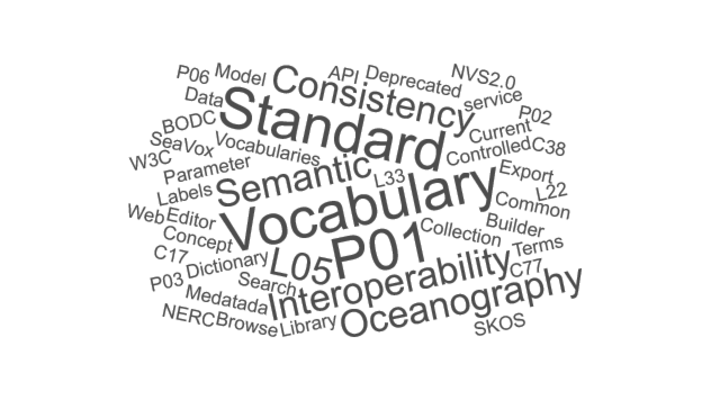
\includegraphics[width=\textwidth]{../episodes/fig/metadata_words.png}
\end{columns}
\end{frame}

% ------------------------------------------------
\begin{frame}{Vocabulários controlados}
\Large
Texto livre pode ser ambíguo:

\vspace{0.3cm}

\centering
\texttt{temp} \quad \texttt{T} \quad \texttt{temperature} \quad \texttt{sea temperature}

\vspace{0.5cm}

\raggedright
Vocabulários controlados resolvem isso usando listas curadas de termos padronizados e identificadores estáveis.

\vspace{0.4cm}

\begin{block}{Benefício}
Diferentes datasets e instituições passam a usar o mesmo conceito quando querem dizer a mesma coisa.
\end{block}
\end{frame}

% ------------------------------------------------
\begin{frame}{NERC Vocabulary Server (NVS)}
\begin{itemize}
  \item Serviço operado pelo British Oceanographic Data Centre (BODC).
  \item Publica vocabulários para dados marinhos e de ciências da Terra.
  \item Inclui termos para parâmetros, instrumentos, plataformas, projetos, regiões e métodos.
  \item Usa identificadores estáveis, permitindo metadados legíveis por máquina.
\end{itemize}

\vspace{0.4cm}

\begin{block}{Exemplo}
Uma variável como ``temperatura da água do mar a 5 m'' pode ser associada a um código P01, reduzindo ambiguidade entre datasets.
\end{block}
\end{frame}

% ------------------------------------------------
\begin{frame}{Padrões importantes}
\begin{table}
\centering
\small
\begin{tabular}{lll}
\toprule
Padrão & Escopo & Papel \\
\midrule
CF Conventions & Dentro do arquivo & Variáveis, unidades, coordenadas \\
ISO 19115 & Dataset como um todo & Descoberta e documentação geográfica \\
INSPIRE & Perfil europeu & Regras para metadados espaciais \\
MEDIN & Perfil marinho do Reino Unido & Descoberta de dados marinhos \\
NVS & Vocabulários & Termos e identificadores estáveis \\
STAC & Catálogo JSON/GeoJSON & Organização de assets no espaço e tempo \\
\bottomrule
\end{tabular}
\end{table}
\end{frame}

% ------------------------------------------------
\begin{frame}{CF metadata conventions}
\Large
As convenções CF definem como descrever dados de ciências da Terra em formatos auto-descritivos, originalmente NetCDF.

\vspace{0.4cm}

CF especifica atributos como:

\begin{itemize}
  \item \texttt{standard\_name};
  \item \texttt{units};
  \item \texttt{cell\_methods};
  \item \texttt{coordinates};
  \item \texttt{bounds};
  \item \texttt{grid\_mapping}.
\end{itemize}
\end{frame}

% ------------------------------------------------
\begin{frame}[fragile]{Exemplo CF em NetCDF}
\begin{lstlisting}[language={}]
sea_surface_temperature:
    standard_name = "sea_surface_temperature"
    units = "K"
    coordinates = "time latitude longitude"
\end{lstlisting}

\vspace{0.4cm}

\begin{block}{Por que isso ajuda?}
Ferramentas como xarray conseguem entender melhor o que a variável representa e como ela se relaciona com as coordenadas do dataset.
\end{block}
\end{frame}

% ------------------------------------------------
\begin{frame}{ISO 19115, INSPIRE e perfis}
\begin{itemize}
  \item ISO 19115 descreve datasets e serviços geográficos.
  \item Inclui identificação, extensão espacial e temporal, qualidade, sistema de referência, responsáveis e distribuição.
  \item INSPIRE define regras de metadados para dados e serviços espaciais no contexto europeu.
  \item Perfis comunitários, como MEDIN e SeaDataNet, adaptam esses padrões a comunidades específicas.
\end{itemize}

\vspace{0.4cm}

\begin{block}{Diferença importante}
CF descreve variáveis dentro do arquivo; ISO e perfis de descoberta descrevem o dataset como um todo.
\end{block}
\end{frame}

% ------------------------------------------------
\begin{frame}[fragile]{Exemplo de metadado de descoberta}
\begin{lstlisting}[language={}]
Title: CTD observations from the North Atlantic, 2025
Organisation: National Oceanography Centre
Geographic extent: 45N-60N, 30W-10W
Temporal extent: 10-25 June 2025
Keywords: ocean temperature, salinity, CTD
Coordinate reference system: WGS 84
Distribution format: NetCDF
\end{lstlisting}
\end{frame}

% ------------------------------------------------
\begin{frame}{WMO: GRIB e BUFR}
\begin{itemize}
  \item A WMO mantém formatos para troca eficiente de dados meteorológicos e oceanográficos.
  \item GRIB é amplamente usado para saídas de previsão numérica do tempo.
  \item BUFR é usado para grandes volumes de observações, como satélites, aeronaves e perfiladores.
  \item Esses formatos são essenciais em centros operacionais.
\end{itemize}

\vspace{0.4cm}

\begin{block}{Conexão com cloud-native}
Mesmo quando os dados operacionais chegam em GRIB ou BUFR, eles podem ser convertidos, catalogados e expostos em fluxos modernos.
\end{block}
\end{frame}

% ------------------------------------------------
\begin{frame}{STAC: SpatioTemporal Asset Catalogs}
\Large
STAC define uma linguagem comum, baseada em JSON/GeoJSON, para descrever e organizar assets geoespaciais no espaço e no tempo.

\vspace{0.4cm}

\begin{itemize}
  \item \textbf{Catalog}: ponto de entrada que conecta coleções e itens.
  \item \textbf{Collection}: conjunto relacionado de dados com metadados compartilhados.
  \item \textbf{Item}: um asset ou produto específico, com links para os arquivos de dados.
\end{itemize}
\end{frame}

% ------------------------------------------------
\begin{frame}{Metadado dentro do arquivo vs metadado de descoberta}
\begin{columns}
\column{0.5\textwidth}
\begin{block}{Dentro do arquivo}
Usado por ferramentas de análise.
\end{block}

\begin{itemize}
  \item \texttt{units};
  \item \texttt{standard\_name};
  \item \texttt{long\_name};
  \item coordenadas;
  \item histórico e proveniência.
\end{itemize}

\column{0.5\textwidth}
\begin{block}{Descoberta}
Usado por catálogos e usuários.
\end{block}

\begin{itemize}
  \item título e resumo;
  \item palavras-chave;
  \item contato;
  \item extensão espacial e temporal;
  \item links de acesso;
  \item licença e citação.
\end{itemize}
\end{columns}
\end{frame}

% ------------------------------------------------
\begin{frame}{Por que os dois são necessários?}
\Large
\begin{block}{Metadados internos}
Permitem que ferramentas como xarray, Iris, CDO e bibliotecas de visualização interpretem arrays corretamente.
\end{block}

\vspace{0.3cm}

\begin{block}{Metadados de descoberta}
Permitem que pessoas, catálogos e APIs encontrem o dataset e decidam se ele serve para uma análise.
\end{block}

\vspace{0.3cm}

\centering
\textbf{Um dataset reutilizável precisa dos dois níveis.}
\end{frame}

% ------------------------------------------------
\begin{frame}{Exercício 1: combine formato e padrão}
Para cada cenário, sugira uma combinação de \textbf{formato + padrão de metadados} e explique o motivo.

\vspace{0.3cm}

\begin{enumerate}
  \item Reanálise global diária de temperatura da superfície do mar em grade regular, publicada para reúso de longo prazo.
  \item Perfis CTD de navio, com metadados detalhados de instrumento, para ingestão em um centro nacional de dados marinhos.
  \item Campos operacionais globais de previsão numérica do tempo disseminados a cada 6 horas.
\end{enumerate}

\vspace{0.4cm}

\begin{block}{Tempo}
5 minutos para pensar ou discutir em pares. Depois compartilhamos as respostas.
\end{block}
\end{frame}

% ------------------------------------------------
\begin{frame}{Possíveis respostas para o exercício 1}
\small
\begin{enumerate}
  \item \textbf{SST em grade}: NetCDF ou Zarr com convenções CF, metadados de descoberta ISO/INSPIRE/MEDIN e, opcionalmente, STAC para expor os assets em um catálogo cloud-native.
  \item \textbf{Perfis CTD}: NetCDF ou CSV com metadados internos ricos, MEDIN para descoberta, e NVS para parâmetros, instrumentos e plataformas.
  \item \textbf{Previsão operacional}: GRIB/GRIB2 com metadados WMO, além de catálogo ou API baseado em ISO/INSPIRE, perfil institucional ou STAC para descoberta.
\end{enumerate}

\vspace{0.3cm}

\begin{block}{Ideia principal}
A melhor escolha depende do tipo de dado, do público, do fluxo operacional e da forma de acesso.
\end{block}
\end{frame}

% ------------------------------------------------
\begin{frame}{Por que seguir padrões?}
\begin{itemize}
  \item \textbf{Interoperabilidade}: ferramentas conseguem ler e interpretar dados sem código customizado.
  \item \textbf{Descoberta}: catálogos conseguem indexar e divulgar datasets.
  \item \textbf{Clareza semântica}: vocabulários reduzem ambiguidade entre instituições.
  \item \textbf{Governança}: padrões ajudam auditoria, documentação, qualidade e manutenção.
  \item \textbf{Eficiência}: reutilizamos ferramentas e infraestruturas existentes em vez de reinventar tudo.
\end{itemize}
\end{frame}

% ------------------------------------------------
\begin{frame}{Padrões no mundo cloud-native}
\Large
Formatos cloud-native não eliminam a necessidade de padrões.

\vspace{0.4cm}

\begin{block}{Pelo contrário}
Quando movemos dados de arquivos locais para object storage, APIs e catálogos, os padrões são o que preservam o significado dos dados.
\end{block}

\vspace{0.4cm}

Zarr, GeoZarr, CF, NVS, ISO e STAC podem trabalhar juntos para conectar o ecossistema científico ao ecossistema geoespacial moderno.
\end{frame}

% ------------------------------------------------
\begin{frame}{Exercício 2: encontre o metadado ausente}
Imagine que você encontra um arquivo \texttt{sst\_daily.nc} com uma variável global de temperatura da superfície do mar.

\vspace{0.3cm}

Dentro do arquivo você vê:

\begin{itemize}
  \item nome da variável: \texttt{temp};
  \item sem atributo \texttt{units};
  \item sem atributo \texttt{standard\_name};
  \item coordenada de tempo sem \texttt{calendar} ou referência como ``days since ...''.
\end{itemize}

\vspace{0.3cm}

\textbf{Que problemas isso pode causar? O que você adicionaria?}
\end{frame}

% ------------------------------------------------
\begin{frame}{Possíveis respostas para o exercício 2}
\begin{itemize}
  \item Sem \texttt{units}, não sabemos se \texttt{temp} está em Kelvin, Celsius ou outra unidade.
  \item Sem \texttt{standard\_name}, ferramentas não reconhecem automaticamente a variável como temperatura da superfície do mar.
  \item Sem metadados de tempo, fica difícil alinhar o dado com outros datasets.
\end{itemize}

\vspace{0.4cm}

\begin{block}{Melhorias mínimas}
Adicionar \texttt{standard\_name="sea\_surface\_temperature"}, \texttt{units="K"}, \texttt{long\_name}, metadados corretos de tempo, título, instituição, resumo, palavras-chave e extensão espacial/temporal.
\end{block}
\end{frame}

% ------------------------------------------------
\begin{frame}{Mensagens principais}
\begin{itemize}
  \item Oceanografia e meteorologia dependem de formatos auto-descritivos, como NetCDF, HDF5 e Zarr, e de formatos operacionais, como GRIB e BUFR.
  \item Metadados existem tanto dentro dos arquivos quanto em registros externos de descoberta.
  \item Vocabulários controlados, como NVS, tornam metadados mais consistentes e legíveis por máquina.
  \item CF descreve variáveis, grades e coordenadas em formatos científicos.
  \item ISO, INSPIRE e MEDIN ajudam na descoberta e documentação de datasets.
  \item STAC organiza assets geoespaciais em fluxos modernos e cloud-native.
\end{itemize}
\end{frame}

% ------------------------------------------------
\begin{frame}{Fechamento}
\Large
Nesta aula, vimos que formatos, metadados e vocabulários não são detalhes administrativos.

\vspace{0.5cm}

\begin{block}{Eles são a base para escala}
Sem padrões, fica difícil automatizar análise, busca, visualização, conversão e acesso remoto.
\end{block}

\vspace{0.4cm}

Na próxima etapa, conectamos essa base ao problema central do curso: trabalhar com dados N-dimensionais grandes em ambientes modernos de processamento e armazenamento.
\end{frame}

\end{document}
